\chapter{Introduction}
\section{Concept}
Goal of the project is to simulate an robotic arm. The robotic arm is drawn in a CAD program called OpenSCAD. This is a sript based CAD program. All the different parts of the robotic arm are exported as a .stl file and then read by the matlab/octave software. That gives us matrizes with pointobjects of all the parts of the arm which can be easily calculated with.\\
The whole project includes five different big parts. First is to draw the robotic arm wish the OpenSCAD software and export the stl files. Second is to include the .stl files into matlab/octave. The third part is to write the code to move all the parts of the robotic arm. The fourth is to dynamically calculate the path to get from point A to point B. And the last part is to test the whole simulation.\\

\section{Schedule}
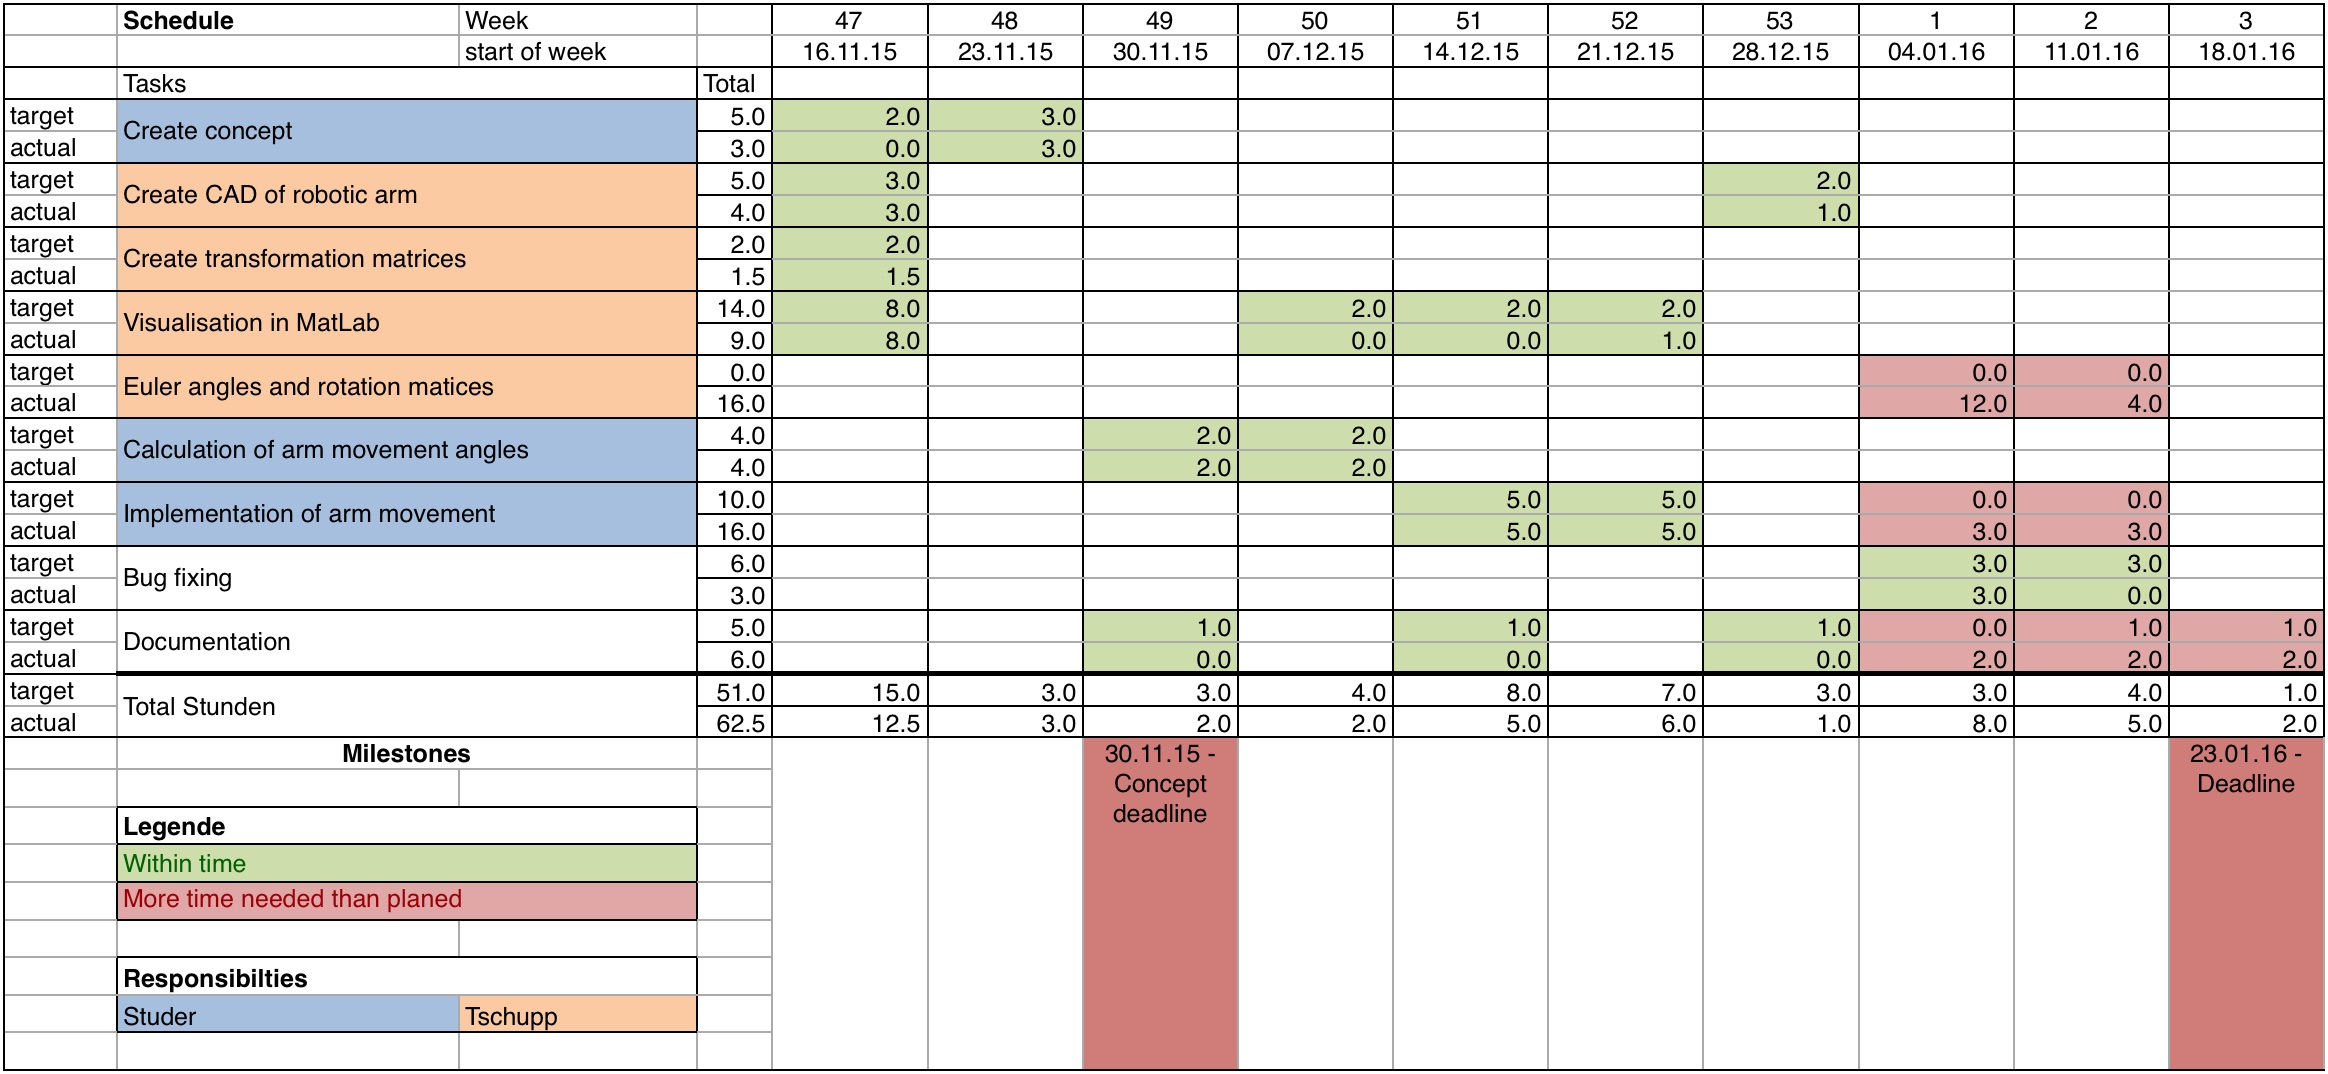
\includegraphics[width=\textwidth]{imgs/schedule.jpg}